\begin{figure}	
	\begin{center}
		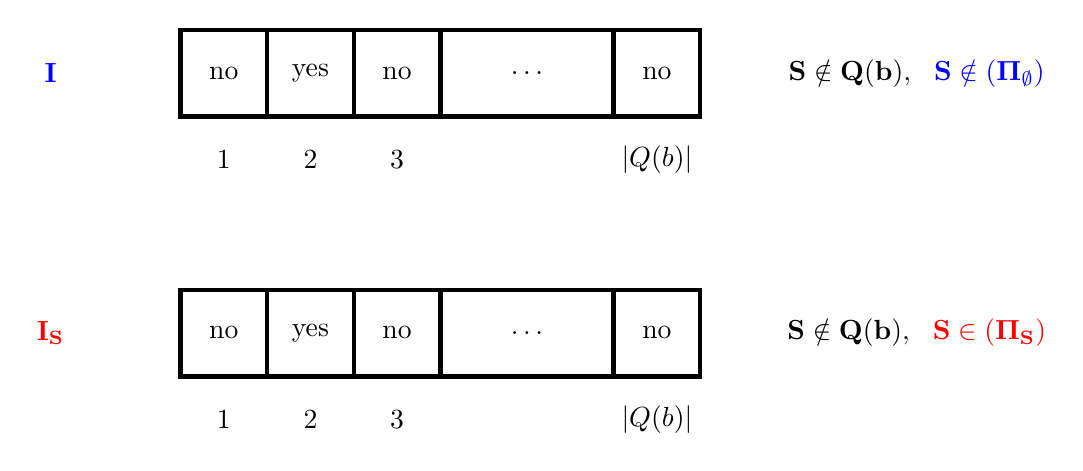
\begin{tikzpicture}[ultra thick,scale=1.1, every node/.style={scale=1}]
		
		
		
		
		\node at (-1.5,3.5) {$\bf \textcolor{blue}{I}$};
		\draw (0,3) rectangle (6,4);
		\draw (1,3)--(1,4);
		\draw (2,3)--(2,4);
		\draw (3,3)--(3,4);
		
		\draw (5,3)--(5,4);
		
		%		\draw (7,0)--(7,1);		
		\draw (6,3)--(6,4);								
		%	\draw (8,3)--(8,4);
		%	\draw (9,3)--(9,4);
		\node at (0.5,2.5) {$1$};
		\node at (0.5,3.5) {no};
		\node at (1.5,2.5) {$2$};
		\node at (1.5,3.5) {yes};
		\node at (2.5,2.5) {$3$};
		\node at (2.5,3.5) {no};
		\node at (4,3.5) {$\ldots$};
		%	\node at (7,3.5) {$\ldots$};
		\node at (5.5,2.5) {$|Q(b)|$};
		\node at (5.5,3.5) {no};
		
		\node at (8.5,3.5) {$\bf \textcolor{black}{S \notin Q(b)},~~ \textcolor{blue}{S \notin \cI(\Pi_{\emptyset})}$};
		%	\node at (10,3.5) {$\ldots$};
		
		%	\node at (8.5,1.3) {$\bf \textcolor{black}{S}$};
		%	\fill[gray, opacity=0.2] (6,3) rectangle (11,4);
		
		% First rectangle I
		\node at (-1.5,0.5) {$\bf \textcolor{red}{I_S}$};
		\draw (0,0) rectangle (6,1);
		\draw (1,0)--(1,1);
		\draw (2,0)--(2,1);
		\draw (3,0)--(3,1);
		
		\draw (5,0)--(5,1);
		
		%	\node at (8.5,4.3) {$\bf \textcolor{black}{S}$};
		
		%		\draw (7,0)--(7,1);		
		\draw (6,0)--(6,1);								
		%			\draw (8,0)--(8,1);
		%	\draw (9,0)--(9,1);
		\node at (0.5,-0.5) {$1$};
		\node at (0.5,0.5) {no};
		\node at (1.5,-0.5) {$2$};
		\node at (1.5,0.5) {yes};
		\node at (2.5,-0.5) {$3$};
		\node at (2.5,0.5) {no};
		\node at (4,0.5) {$\ldots$};
		%	\node at (10,0.5) {$\ldots$};
		%	\node at (7,0.5) {$\ldots$};
		\node at (5.5,-0.5) {$|Q(b)|$};
		\node at (5.5,0.5) {no};
		
		\node at (8.5,0.5) {$\bf \textcolor{black}{S \notin Q(b)},~~ \textcolor{red}{ S \in \cI(\Pi_{S})}$};
		
		
		%	\node at (8.5,1.3) {$\bf \textcolor{black}{S}$};
		%	\fill[gray, opacity=0.2] (6,0) rectangle (11,1);
		%	\node at (0.5,-0.5) {$\x$};
		%		\foreach \x in {1,2,3,4,5,6,7,8,9}{
		%			\draw (\x,0)--(\x,1);
		%			\node at (\x-0.5,-0.5) {$\x$};
		%		}
		%		\node at (10.5,-0.5) {$\ldots$};
		%		\node at (11.5,-0.5) {$Q()b$};
		
		% Second rectangle I_S
		%		\node at (-1,-2.5) {$I_S$};
		%		\draw (0,-3) rectangle (10,-2);
		%		\foreach \x in {1,2,3,4,5,6,7,8,9}{
		%			\draw (\x,-3)--(\x,-2);
		%			\node at (\x-0.5,-3.5) {$\x$};
		%			\node at (\x-0.5,-2.5) {no};
		%		}
		%		\node at (10.5,-3.5) {$\ldots$};
		%		\node at (11.5,-3.5) {$x$};
		%		\node at (11.5,-2.5) {yes};
		%		\node at (11.5,-1.5) {$S$};
		
		\end{tikzpicture}
	\end{center}
	\caption{\label{fig:proof} An illustration of the proof of \Cref{thm:emb}. The figure presents the sequences of queries to the membership oracles by the algorithm on the instances $I$ and $I_S$ for a string of bits $b$, such that $S \notin Q(b)$. The label ''yes" (''no") indicates that the queried set is (not) independent in the matroid. 
		The only query that distinguishes between $I$ and $I_S$ is on the set $S$, which is not queried; thus, the algorithm returns the same output for $I$ and $I_S$.}
\end{figure}


\thmemb*
	\begin{proof}
		Assume towards contradiction that there exist a constant $d \in \mathbb{N}$ and a randomized algorithm $\cA$ that decides every oracle-EMB instance $(E,\cI,c,T)$ in time $\left( (T+2) \cdot n \cdot m \right)^{d}$, where $n = |E|+1$ and $m = c(E)+1$.  
		For every $n,k,\alpha \in \mathbb{N}_{>0}$, consider the set of all subsets of $[n]$ with cardinality $k$ and sum $\alpha$: $$\mathcal{F}_{n,k,\alpha} = \big\{S \subseteq [n]~\big|~|S| = k, \textnormal{\textsf{sum}}(S) = \alpha\big\}.$$ 
		To reach a contradiction, we construct an induced oracle-EMB instance on which $\cA$ does not compute the proper output with sufficiently high probability. The parameters of the instance are extracted from the following combinatorial claim. 
			\begin{claim}
			\label{claim:H1}
			There are $\tilde{n} \in \mathbb{N}_{>0}$, $\tilde{k} \in \left[\tilde{n}\right]$, and $\tilde{\alpha} \in \left[\tilde{n}^2\right]$ such that 
$|\mathcal{F}_{\tilde{n},\tilde{k},\tilde{\alpha}}|> 	2 \cdot \left(	12 \cdot \tilde{n}^5 \right)^{d} $. 
%the following holds
%			\begin{equation*}
%				\begin{aligned}
%						\left(	12 \cdot \tilde{n}^5 \right)^{d} < \frac{2^{\tilde{n}}-1}{2 \cdot \left(\tilde{n}+1\right) \cdot \tilde{n}^2},~~~~~~~~~~~~~	{\tilde{n} \choose \tilde{k}} \geq \frac{2^{\tilde{n}}-1}{\tilde{n}+1}, ~~~~~~~~~~~~~ |\mathcal{F}_{\tilde{n},\tilde{k},\tilde{\alpha}}| \geq  \frac{{\tilde{n} \choose \tilde{k}}}{\tilde{n}^2}. 
%				\end{aligned}
%			\end{equation*}
		\end{claim}
		\begin{claimproof}
				Since $d$ is a constant, %it holds that $$\lim_{n \rightarrow \infty}  \frac{\left(\frac{2^{n}-1}{2 \cdot \left(n+1\right) \cdot n^2}\right)}{\left(	8 \cdot n^5 \right)^{d}} = \infty.$$ Thus, 
				there is $\tilde{n} \in \mathbb{N}_{>0}$ such that 
				\begin{equation}
					\label{eq:nTild}
						\left(	12 \cdot \tilde{n}^5 \right)^{d} < \frac{2^{\tilde{n}}-1}{2 \cdot \tilde{n}^3}.
				\end{equation}
				  Fix $\tilde{n} \in \mathbb{N}_{>0}$ satisfying \eqref{eq:nTild}. Recall that $\sum_{k \in \{0,1,\ldots,\tilde{n}\}} {\tilde{n} \choose k} = 2^{\tilde{n}}$ from a basic property of the Pascal triangle; therefore, $\sum_{k \in \{1,\ldots,\tilde{n}\}} {\tilde{n} \choose k} = 2^{\tilde{n}}-1$. Thus, there is  $\tilde{k} \in \{1,\ldots,\tilde{n}\}$, 
				  such that 
				  \begin{equation}
				  	\label{eq:kTild}
				  	{\tilde{n} \choose \tilde{k}} \geq \frac{2^{\tilde{n}}-1}{\tilde{n}}.
				  \end{equation}
				   Fix $\tilde{k} \in \left[\tilde{n}\right]$ satisfying \eqref{eq:kTild}. Observe that for each $S \in 2^{[\tilde{n}]}$ satisfying $|S| = \tilde{k}>0$, it holds that $1 \leq \textnormal{\textsf{sum}}(S) \leq |S| \cdot \max_{i \in [\tilde{n}]} i = \tilde{n}^2$. Thus, there are $\tilde{n}^2$ possibilities for $\alpha \in \left[\tilde{n}^2\right]$ satisfying $\alpha = \textnormal{\textsf{sum}}(S)$, for some $S \in 2^{[\tilde{n}]}$ such that $|S| = \tilde{k}$. Moreover, there are ${\tilde{n} \choose \tilde{k}}$ subsets of $[\tilde{n}]$ of cardinality $\tilde{k}$. By the pigeonhole principle, there is $\tilde{\alpha} \in  \left[  \tilde{n}^2 \right]$ such that $|\mathcal{F}_{\tilde{n},\tilde{k},\tilde{\alpha}}| \geq  \frac{{\tilde{n} \choose \tilde{k}}}{\tilde{n}^2}$. Thus,
				   $$|\mathcal{F}_{\tilde{n},\tilde{k},\tilde{\alpha}}| \geq \frac{{\tilde{n} \choose \tilde{k}}}{\tilde{n}^2}  \geq  \frac{2^{\tilde{n}}-1}{\tilde{n} \cdot \tilde{n}^2} > 2 \cdot \left(	12 \cdot \tilde{n}^5 \right)^{d}.$$ The second inequality follows from \eqref{eq:kTild}, and the third inequality holds by \eqref{eq:nTild}. 
		\end{claimproof}
		
	

		
		Let $\tilde{n} \in \mathbb{N}_{>0}$, $\tilde{k} \in \left[\tilde{n}\right]$, and $\tilde{\alpha} \in \left[\tilde{n}^2\right]$  satisfying the conditions of \Cref{claim:H1}. Define $t$ to be the maximum running time of $\cA$ on an induced EMB instance $I_{\tilde{n},\tilde{k},\tilde{\alpha}}(\Pi)$ over all $\Pi \in 2^{\left[ \tilde{n}\right]}$. 
			\begin{claim}
			\label{claim:H2}
			$t \leq	\left(	12 \cdot \tilde{n}^5 \right)^{d}$.    
		\end{claim}
		\begin{claimproof}
				Let $T = \tilde{\alpha}$, $n = \tilde{n}+1$, and $m = \textsf{id}_{\tilde{n}}(\left[\tilde{n}\right])+1$. By the running time guarantee of $\cA$, it follows that $t \leq	\left(	n \cdot (T+2) \cdot m \right)^{d}$. It remains to bound $n \cdot (T+2) \cdot m$. Since $\textsf{id}_{\tilde{n}}(\left[\tilde{n}\right]) = \textsf{sum}(\left[\tilde{n}\right])$ and $\tilde{\alpha} \leq \tilde{n}^2$, %By the definition of induced EMB instance (\Cref{def:EMBpi}) with parameters $\tilde{n},\tilde{k},\tilde{\alpha}$,
				 \begin{equation*}
				\label{eq:InducedParameters}
				%(\tilde{\alpha} +1) \cdot \left( \textsf{id}_{\tilde{n}} ( \left[\tilde{n} \right])+1 \right) \cdot \left(\tilde{n}+1\right) 
				n  \cdot (T+2) \cdot m \leq	 \left(\tilde{n}+1\right) \cdot \left( \tilde{n}^2+2\right)\left( \textsf{sum}( \left[\tilde{n} \right])+1 \right) \leq 2 \tilde{n} \cdot 3 \tilde{n}^2 \cdot \left(\frac{\tilde{n} \cdot (\tilde{n}+1)}{2}+1 \right) \leq 12 \cdot \tilde{n}^5. 
			\end{equation*}  The second inequality follows from the sum of the terms of an arithmetic sequence. By the above and the running time guarantee of $\cA$, it follows that $t \leq	\left(	n \cdot (T+2) \cdot m \right)^{d} \leq 	\left(	12 \cdot \tilde{n}^5 \right)^{d}$.   
		\end{claimproof}
		
	Given  an induced oracle-EMB instance $I_{\tilde{n},\tilde{k},\tilde{\alpha}}(\Pi)$, for some $\Pi \subseteq \left[ \tilde{n}\right]$,  the randomized algorithm $\cA$ produces a random string of bits $\bar{b} \in \{0,1\}^{t}$ and performs a sequence of queries to the membership oracle of $M_{\tilde{n},\tilde{k},\tilde{\alpha}}$, based on $\bar{b},\tilde{n},\tilde{k},\tilde{\alpha}$, and the results of the previous queries; then, the algorithm decides the given instance based on the queries. 
		 
		 
		 Let $\Pi_{\emptyset} = \emptyset$, and consider the induced oracle-EMB instance $I = I_{\tilde{n},\tilde{k},\tilde{\alpha}}(\Pi_{\emptyset})$. Given a string of bits $b \in \{0,1\}^{t}$, let $Q(b) \subseteq 2^{[\tilde{n}]}$ be the set of  all subsets $S \subseteq [\tilde{n}]$ queried by $\cA$ on the instance $I$ and the bit-string $b$ (on the membership oracle of $M_{\tilde{n},\tilde{k},\tilde{\alpha}}(\Pi_{\emptyset})$). For clarity, we use $\bar{b}$ for a random string, and $b$ for a realization of $\bar{b}$ to a specific string. Note that $Q(b)$ is a set, since the algorithm is deterministic for every $b \in \{0,1\}^{t}$; conversely, $Q(\bar{b})$ is a random set for a random string $\bar{b} \in \{0,1\}^{t}$. As the running time of $\cA$ on %an induced EMB instance with $\tilde{n}$ elements and rank parameter $\tilde{k}$ 
		$I$ is bounded by $t$, it holds that $|Q(b)| \leq t$ for every $b \in \{0,1\}^{t}$. Let 
		\begin{equation*}
			\label{eq:R}
			R(I) = \left\{S \in \mathcal{F}_{\tilde{n},\tilde{k},\tilde{\alpha}}~\bigg|~\Pr \left(S \in Q(\bar{b}) \right) \geq \frac{1}{2} \right\}
		\end{equation*} be all sets in $ \mathcal{F}_{\tilde{n},\tilde{k},\tilde{\alpha}}$ that are queried by $\cA$ with probability  at least $\frac{1}{2}$. 
			\begin{claim}
			\label{claim:H3}
			$|R(I)|  < |\mathcal{F}_{\tilde{n},\tilde{k},\tilde{\alpha}}|$. 
		\end{claim}
		\begin{claimproof}
			By the definition of $R(I)$, it holds that 
				\begin{equation*}
				\label{eq:R0}
				\begin{aligned}
					|R(I)| ={} & \left| \left\{S \in \mathcal{F}_{\tilde{n},\tilde{k},\tilde{\alpha}}~\bigg|~\Pr \left(S \in Q(\bar{b}) \right) \geq \frac{1}{2} \right\} \right| \\
					\leq{} & 2 \cdot \sum_{S \in \mathcal{F}_{\tilde{n},\tilde{k},\tilde{\alpha}}} \Pr \left(S \in Q(\bar{b}) \right)  \\
					={} & 	 2 \cdot \sum_{S \in \mathcal{F}_{\tilde{n},\tilde{k},\tilde{\alpha}}~} \sum_{b \in \{0,1\}^{t}} \Pr \left(S \in Q(b) \right) \cdot \Pr(\bar{b} = b)
				\end{aligned}
			\end{equation*} Thus, by changing the order of summation, we have 
				\begin{equation*}
				\begin{aligned}
					|R(I)| \leq 2 \cdot  \sum_{b \in \{0,1\}^{t}~} \Pr(\bar{b} = b) \cdot \sum_{S \in \mathcal{F}_{\tilde{n},\tilde{k},\tilde{\alpha}}} \Pr \left(S \in Q(b) \right) 
					\leq 2 \cdot  \sum_{b \in \{0,1\}^{t}~} \Pr(\bar{b} = b) \cdot |Q(b)| .
				%	\leq {} &  2  t \cdot \sum_{b \in \{0,1\}^{t}~} \Pr (\bar{b} = b).
				\end{aligned}
			\end{equation*} 
			
Since $\left|Q(b)\right| \leq t$ for all $b \in \{0,1\}^t$, by the above we have
			\begin{equation*}
				|R(I)| 	\leq 2  t \cdot \sum_{b \in \{0,1\}^{t}~} \Pr (\bar{b} = b) = 2  \cdot t \leq 2\cdot	\left(	12 \cdot \tilde{n}^5 \right)^{d} 
		%		<   \frac{2^{\tilde{n}}-1}{\left(\tilde{n}+1\right) \cdot \tilde{n}^2} \leq  \frac{{\tilde{n} \choose \tilde{k}}}{\tilde{n}^2} 
				< |\mathcal{F}_{\tilde{n},\tilde{k},\tilde{\alpha}}|. 
			\end{equation*}
			The second inequality follows from \Cref{claim:H2}. The last inequality holds by \Cref{claim:H1}. 
		\end{claimproof}
	
	By \Cref{claim:H3}, there exists $S \in F_{\tilde{n},\tilde{k},\tilde{\alpha}} \setminus R(I)$. %; thus, $\Pr \left( S \in Q(\bar{b}) \right) < \frac{1}{2}$. Now, 
		Consider the induced oracle-EMB instance %$I_S = (\tilde{n},\tilde{k},\alpha,M_{\tilde{n},\tilde{k},\alpha}(\Pi_{S}))$ 
		$I_S = I_{\tilde{n},\tilde{k},\tilde{\alpha}}(\Pi_S)$ where $\Pi_{S} = \{S\}$, and let $B = \{b \in \{0,1\}^t~|~ S \notin Q(b)\}$ be all strings for which $S$ is not queried by $\cA$ on the instance $I$ .
	Observe that for all $b \in B$ it holds that the answers to all queries for $T \in Q(b)$ are the same for both oracles (of $M_{\tilde{n},\tilde{k},\tilde{\alpha}}(\Pi_{\emptyset})$ and $M_{\tilde{n},\tilde{k},\tilde{\alpha}}(\Pi_{S})$). Moreover, the decision on which set to query next depends only on $b,\tilde{n},\tilde{k},\tilde{\alpha}$, and the answers to previous queries.  
	
	Hence, for all $b \in B$,  the executions of $\cA$ on the instances $I$ and $I_S$ are identical.
		Since $\Pi_{\emptyset} = \emptyset$, by %\eqref{eq:1} and \Cref{def:EMBpi} 
		\Cref{obs:YesNo}, $I$ is a ``no''-instance for oracle-EMB; thus, $\cA$ returns that $I_S$ is a ``no''-instance for every $b\in B$. However, since $\textsf{id}_n(S) = \textsf{sum}(S) = \alpha$, $|S| = k$, and $S \in \Pi_{S}$, it follows that $I_S$ is a ``yes''-instance by \Cref{obs:YesNo}.  
%		does not query the membership oracle of $M_{\tilde{n},\tilde{k},\alpha}(\Pi_{S})$ with $S$; %The reason is that the answers to all queries in $Q(b)$ are the same for both oracles (of $M_{n,k,\alpha}(\Pi_{\emptyset})$ and $M_{n,k,\alpha}(\Pi_{S})$), and the decision which sets to query next depends only on $b,n,k,\alpha$, and the answers to previous queries.  
		%
		% $Pr[\bar{b} = b] = Pr[b(I_S) = b]$ since the inputs $I$ and $I_S$ are completely similar besides the membership oracle. Thus, $Pr[S \in Q(b(I_S))] = Pr[S \in Q(\bar{b})] < \frac{1}{2}$. 
		%
		Therefore, $\cA$ does not decide $I_S$ correctly for all $b \in B$.  We give an illustration in \Cref{fig:proof}. Since  $S \notin R(I)$, it holds that $\Pr \left( \bar{b} \in B \right) = \Pr \left(S \notin Q(\bar{b}) \right) > \frac{1}{2}$; thus, with probability greater than $\frac{1}{2}$, $\cA$ does not decide correctly the instance $I_S$. 
		%
		%Therefore, w.p. strictly larger than $\frac{1}{2}$ algorithm $\cA$ does not query $S$ for the instance $I_S$. Hence, w.p. strictly larger than $\frac{1}{2}$ algorithm $\cA$ performs the exact same computations on $I$ and $I_S$ and must return the same result. %Note that if the algorithm does not query $S$ it cannot decide correctly the instance $I_S$, since $S$ is the unique solution of $I_S$. 
		%Since $\mathcal{L}_{n,k,\alpha}(\Pi_{\emptyset}) = \emptyset$ and $\mathcal{L}_{n,k,\alpha}(\Pi_{S}) \neq \emptyset$, we conclude that algorithm $\cA$ cannot decide correctly w.p. at least $\frac{1}{2}$ both $I$ and $I_S$, which 
		A contradiction to the correctness of  $\cA$  as a randomized algorithm for oracle-EMB. The statement of the theorem follows. 
	\end{proof}
	
	
	
	

	